\subsection{Including partial top quark mass effects}

%\textit{Authors:} Ajjath A H, Long-Bin Chen, Hai Tao Li, Hua-Sheng Shao, Jian Wang (1912.13001, 2209.03914)

\textbf{Ajjath A H, Long-Bin Chen, Xuan Chen, Yuesheng Dai, Hai Tao Li, Shi-Yuan Li, Hua-Sheng Shao, Jian Wang~\cite{Chen:2019fhs,Ajjath:2022kpv,Chen:2026zmi}.}

\noindent Since finite top quark mass effects cannot be neglected and are exactly known only at NLO~\cite{Borowka:2016ehy,Borowka:2016ypz,Baglio:2018lrj,Davies:2019dfy}, we improve the NLO QCD computation with full top quark mass dependence~\cite{Heinrich:2017kxx,Heinrich:2019bkc,Davies:2025qjr} (denoted as ``$\NLOmt$") by multiplying it with the higher-order (differential) $K$-factors calculated in the HTL in this subsection. The reweighting is carried out consistently using the on-shell top quark mass scheme in $\NLOmt$ and the on-shell mass in the HTL predictions. The resulting combinations are denoted as $\NkLOtimesNLOmt$ and $\NkLONkLLtimesNLOmt$, where $k$ is a positive integer. Specifically,
\begin{eqnarray}\label{NkLO-fullmt}
d\sigma_{\NkLOtimesNLOmt}&\equiv& d\sigma_{\NLOmt}\frac{d\sigma_{\NkLO}}{d\sigma_{\rm NLO}}\,,\nonumber\\
d\sigma_{\NkLONkLLtimesNLOmt}&\equiv&d\sigma_{\NLOmt}\frac{d\sigma_{\NkLONkLL}}{d\sigma_{\rm NLO}}\,.
\end{eqnarray}
This treatment is justified under certain working assumptions; alternative approaches to incorporating top quark mass effects can be found in Section~3 of Ref.~\cite{Chen:2019fhs}.




\begin{sloppypar}
The inclusive phase-space-integrated cross sections are listed in Table~\ref{Tab:fullMt_inc} for LHC $pp$ collisions at $\sqrt{s}=14$ TeV and for five perturbative orders: $\NLOmt$, $\NNLOtimesNLOmt$, $\NNLONNLLtimesNLOmt$, $\NtLOtimesNLOmt$, and $\NtLONtLLtimesNLOmt$. The N$^3$LO QCD corrections enhance the $\NLOmt$ cross section by $21\%$. The N$^3$LL threshold resummation only marginally modifies the $\NtLOtimesNLOmt$ cross section. The scale uncertainty is significantly reduced when higher-order QCD corrections are included: the width of the uncertainty band from the envelope of the $7$-point scale variation in $\NtLOtimesNLOmt$ is only about one quarter of that in the previous fixed-order $\NNLOtimesNLOmt$ result. Inclusion of N$^3$LL threshold resummation further reduces the scale uncertainty to below one percent. A similar pattern is observed in the differential invariant-mass distribution of the Higgs boson pair, as shown in the left panel of Fig.~\ref{fig:xs_vs_mhh_large_mt1}.
\end{sloppypar}

With the fiducial cuts defined in Eq.~\eqref{eq:fiducialcuts}, only fixed-order predictions are given in Table~\ref{Tab:fullMt_inc}, as fully differential soft-gluon resummation predictions are not available. The N$^3$LO QCD corrections enhance the $\NLOmt$ cross section by $18\%$, which is close to the inclusive case. The $m_{hh}$ distribution with fiducial cuts, shown in the right panel of Fig.~\ref{fig:xs_vs_mhh_large_mt1}, highlights the necessity of including finite top quark mass effects. A similar behaviour is seen in the $p_T$ distributions of the leading and subleading Higgs bosons in Figs.~\ref{fig:fid_pth1_mt} and~\ref{fig:fid_pth2_mt}. For more detailed discussions, we refer the interested reader to Ref.~\cite{Chen:2026zmi}.



\begin{table}%[ht] 
\begin{center}

% \begin{small}
\newcolumntype{P}[1]{>{\centering\arraybackslash}m{#1}}
{\renewcommand{\arraystretch}{1.5}
%\begin{tabular}{|P{4cm}|P{3cm}|}
\resizebox{0.98\textwidth}{!}{%
\begin{tabular}{P{5cm}P{5cm}P{5cm}}
%\hline
    \toprule
        Contributions   &Inclusive cross section [$\textup{fb}$]  &Fiducial cross section [$\textup{fb}$] \\
    \midrule
%    $\sigma_{\NLOmt}$ & $32.64_{-12.5\%}^{+13.5\%}~\textup{fb}$\\
    $\NLOmt$ & $32.64_{-12.5\%}^{+13.5\%}$  &  $28.44_{-12 \%}^{+14 \%}$ \\
%     \hline
%    $\sigma_{\NNLOtimesNLOmt}$ & $38.42_{-7.6\%}^{+5.2\%}~\textup{fb}$\\
    $\NNLOtimesNLOmt$ & $38.42_{-7.6\%}^{+5.2\%}$ & $33.40_{-7.3 \%}^{+5.2 \%}$ \\
%    \hline
%   $\sigma_{\NNLONNLLtimesNLOmt}$ & $39.42_{-3.4\%}^{+3.0\%}~\textup{fb}$    \\
   $\NNLONNLLtimesNLOmt$ & $39.42_{-3.4\%}^{+3.0\%}$  & -  \\
%    \hline
%    $\sigma_{\NtLOtimesNLOmt}$ & $39.56_{-2.7\%}^{+0.50\%}~\textup{fb}$ \\  
    $\NtLOtimesNLOmt$ & $39.56_{-2.7\%}^{+0.50\%}$ & $34.68(4)^{+1.4\%}_{-2.9\%}$ \\  
%    \hline
%    $\sigma_{\NtLONtLLtimesNLOmt}$ &  $39.60_{-0.87\%}^{+0.85\%}~\textup{fb}$ \\
    $\NtLONtLLtimesNLOmt$ &  $39.60_{-0.87\%}^{+0.85\%}$ & - \\
% \hline
%  \hline
    \bottomrule
\end{tabular}}}
\caption{Inclusive and fiducial phase-space-integrated cross sections for Higgs boson pair production via gluon fusion at $\sqrt{s}=14\,\textup{TeV}$ in $pp$ collisions, including top quark mass effects. The quoted relative uncertainties correspond to $7$-point scale variations.}
\label{Tab:fullMt_inc}
\end{center}
\end{table}

\begin{figure*}[!htbp]
\centering
\vspace{-1.5cm}
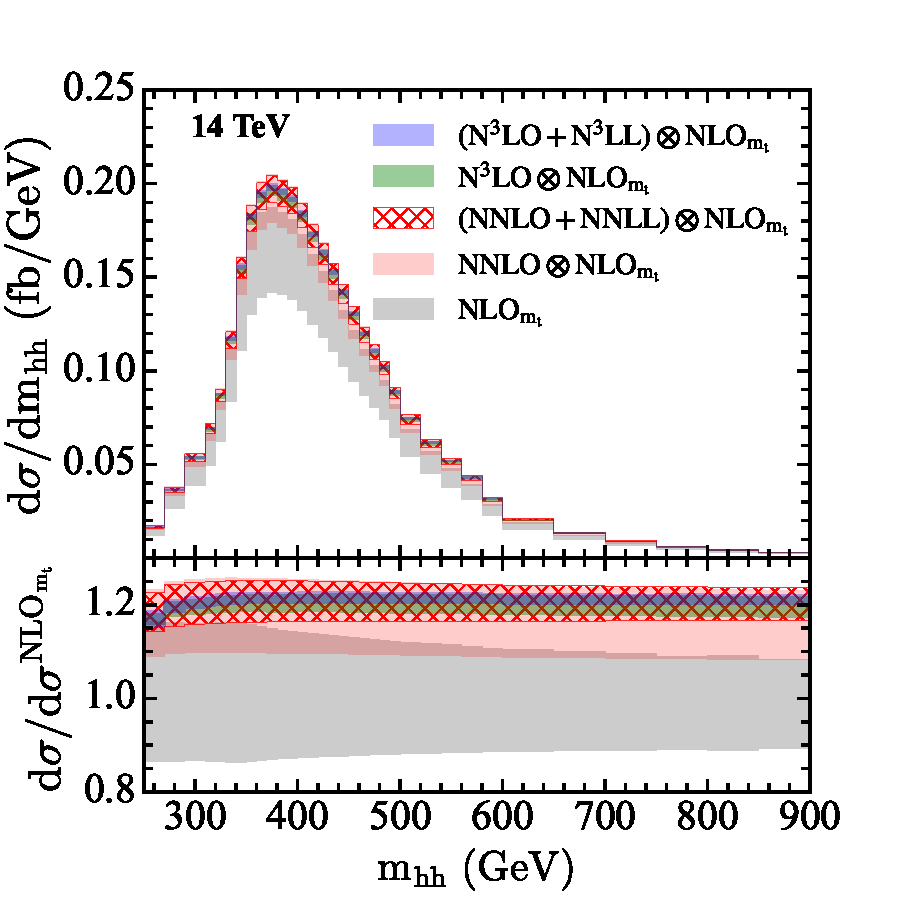
\includegraphics[width=0.49\textwidth]{N3LO_QCD_SM/N3LO_mt/Images/diff_full_mt_13_14_CERNYR5}
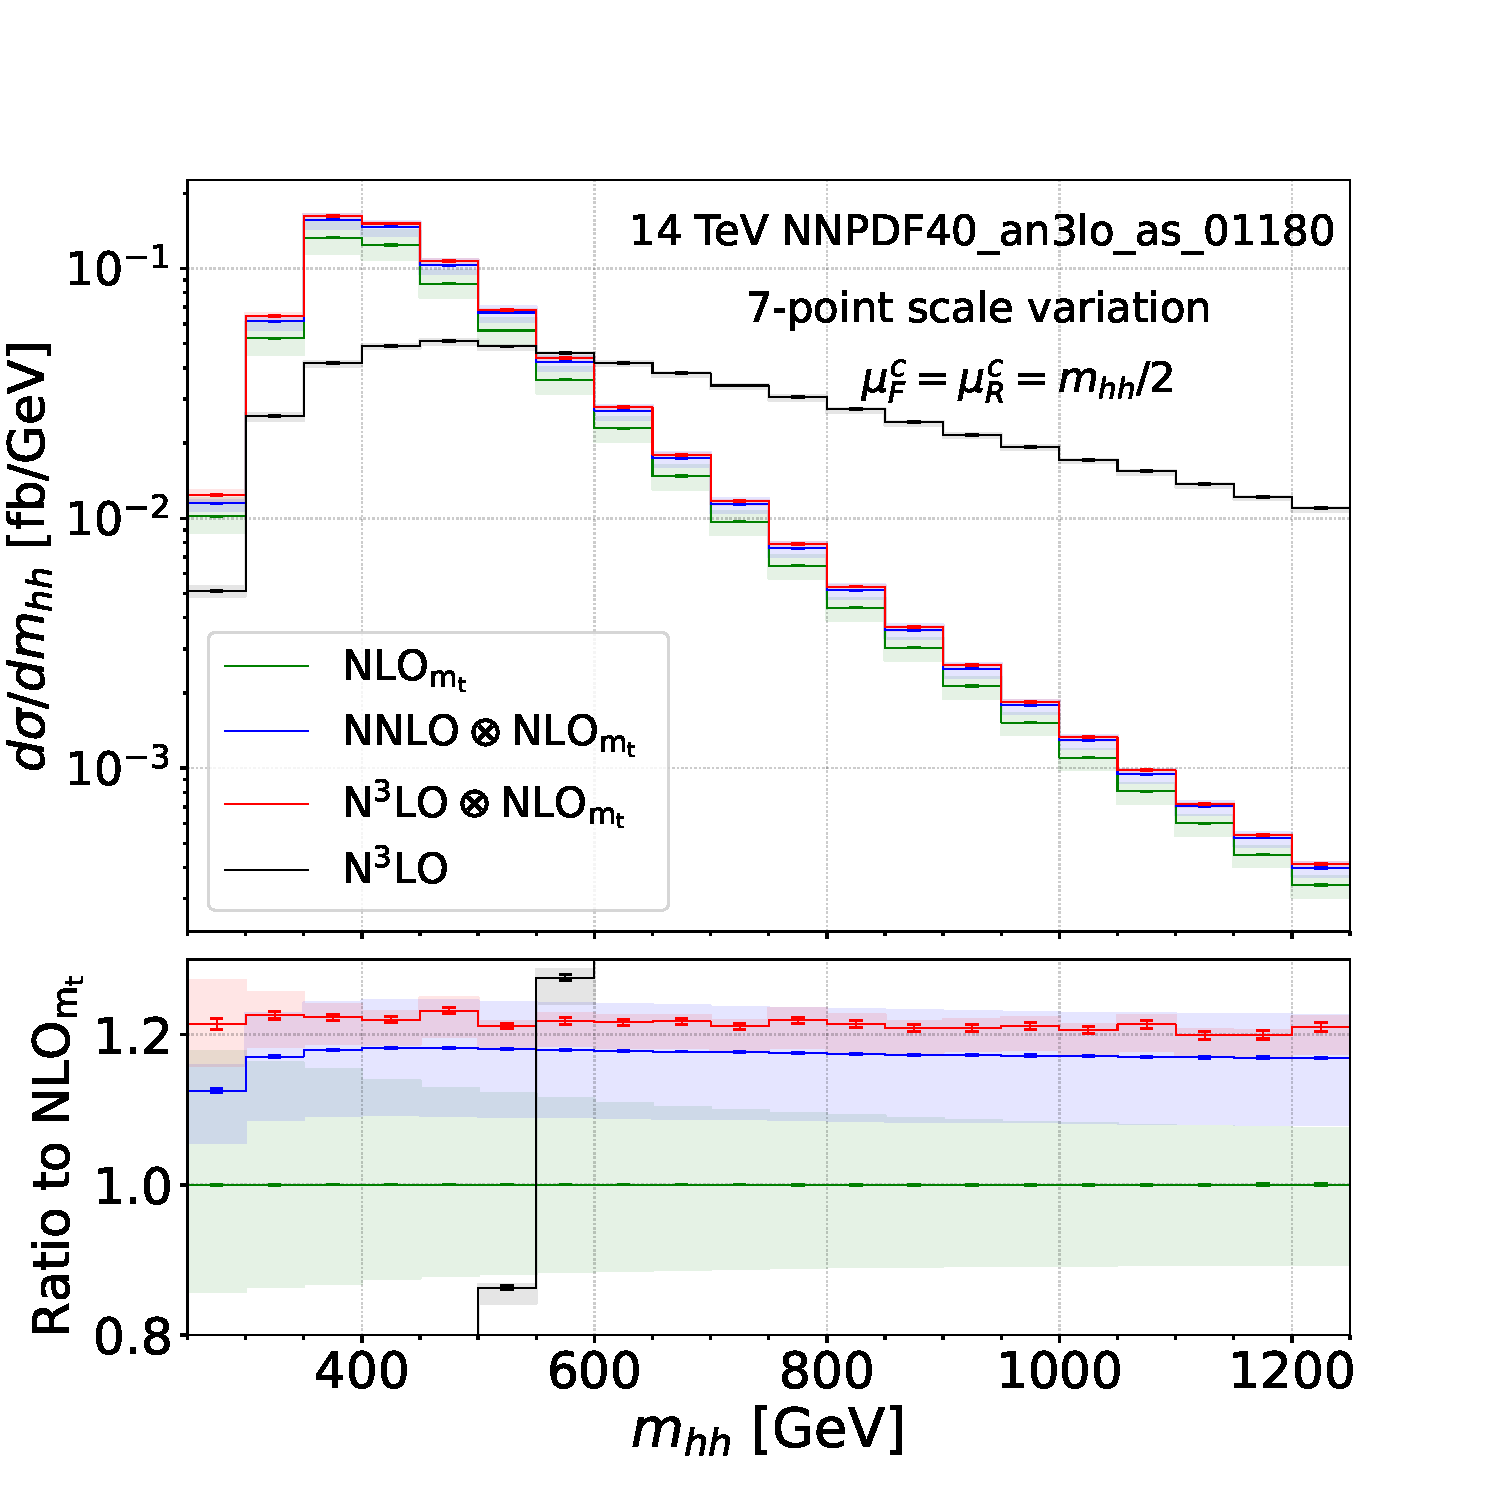
\includegraphics[width=0.49\textwidth,height=7.52cm]{N3LO_QCD_SM/N3LO_mt/Images/HH_m_hh_r}
\\
\caption{Inclusive (left) and fiducial (right) invariant-mass distributions for Higgs boson pair production at $\sqrt{s}=14$ TeV, including top quark mass effects. The error bands stem from $7$-point scale variations. Here $\mu^C$ denotes the central value of the renormalization and factorization scales. Results shown are from Refs.~\cite{Chen:2019fhs,Ajjath:2022kpv,Chen:2026zmi}.}
\label{fig:xs_vs_mhh_large_mt1}
\end{figure*}



\begin{figure*}[h]
\centering
\vspace{-2cm}
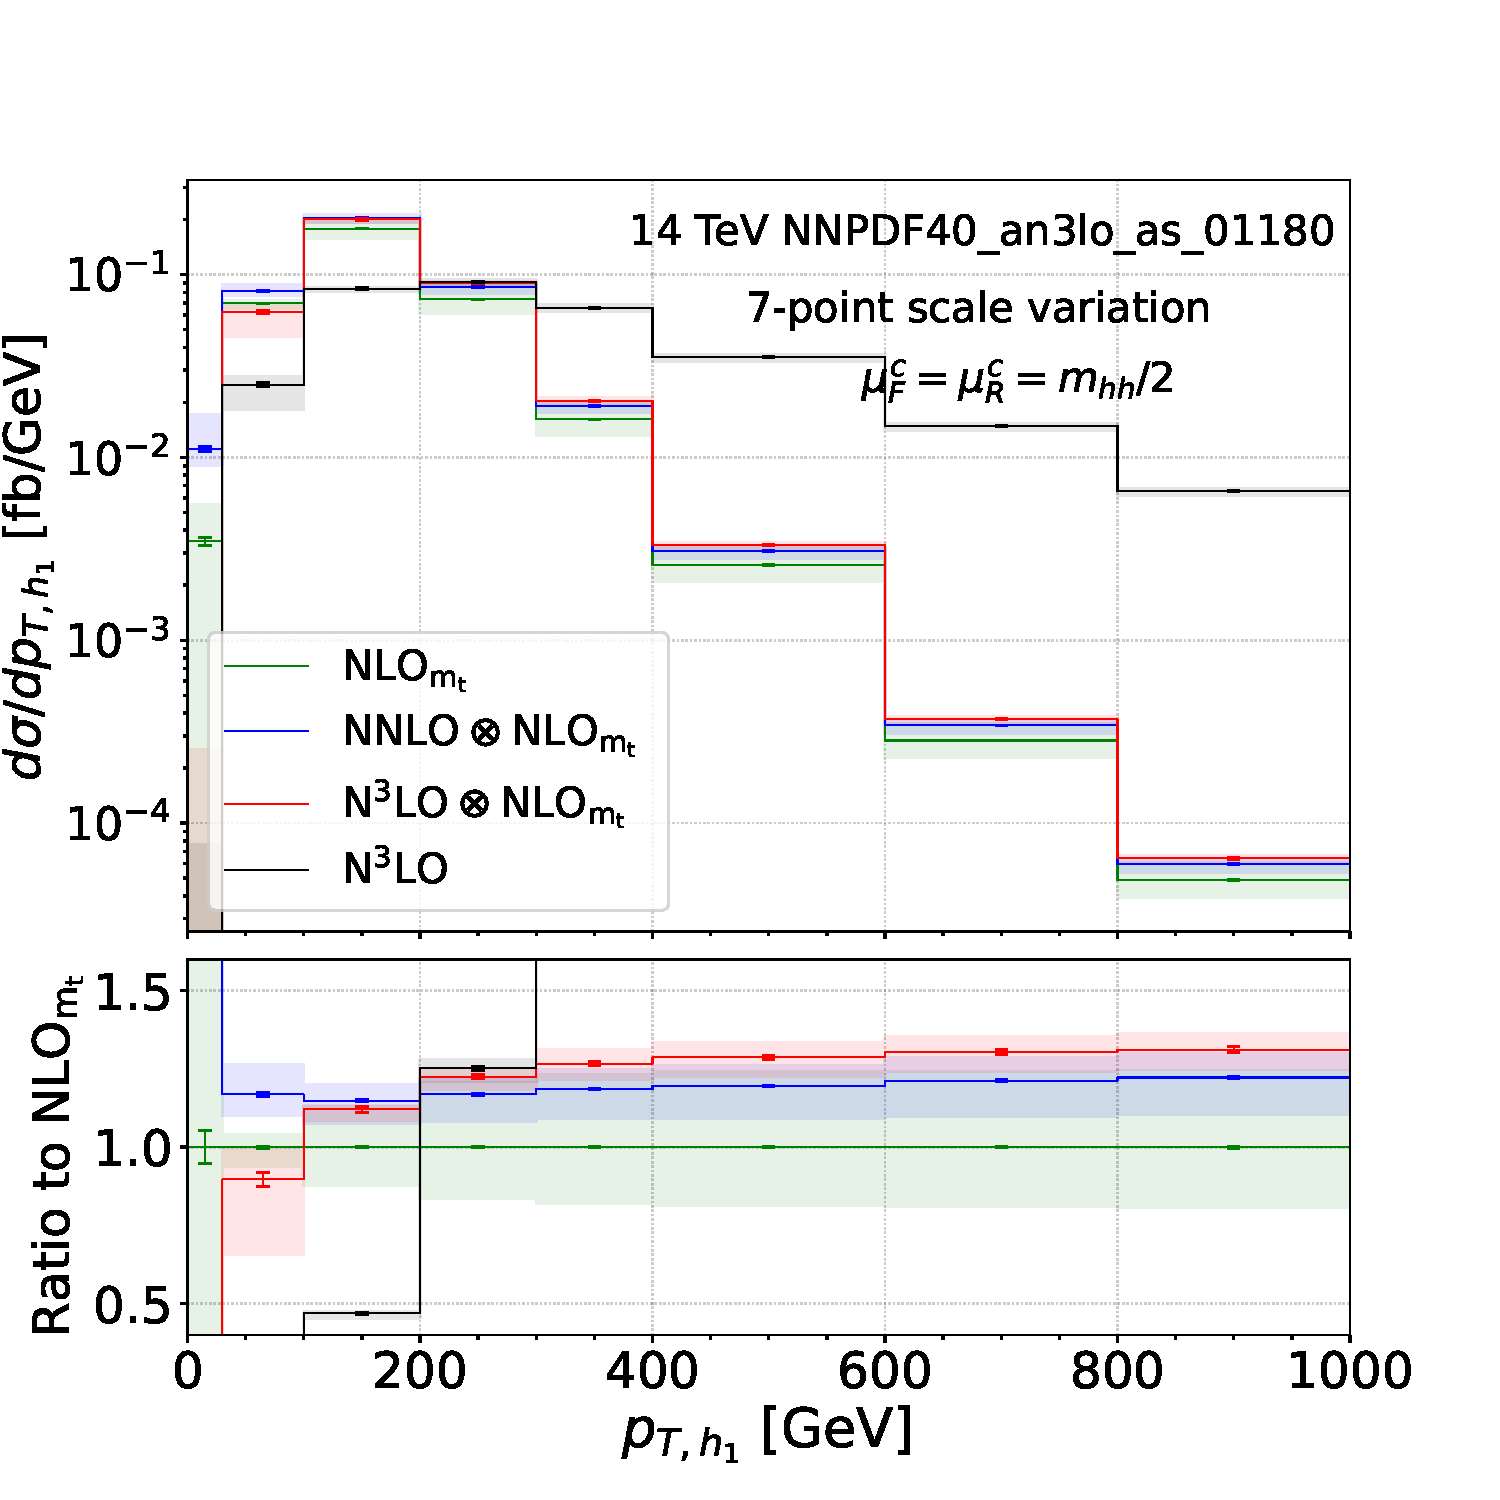
\includegraphics[width=0.49\textwidth,height=7.52cm]{N3LO_QCD_SM/N3LO_mt/Images/HH_pt_h1st_100_r.pdf}
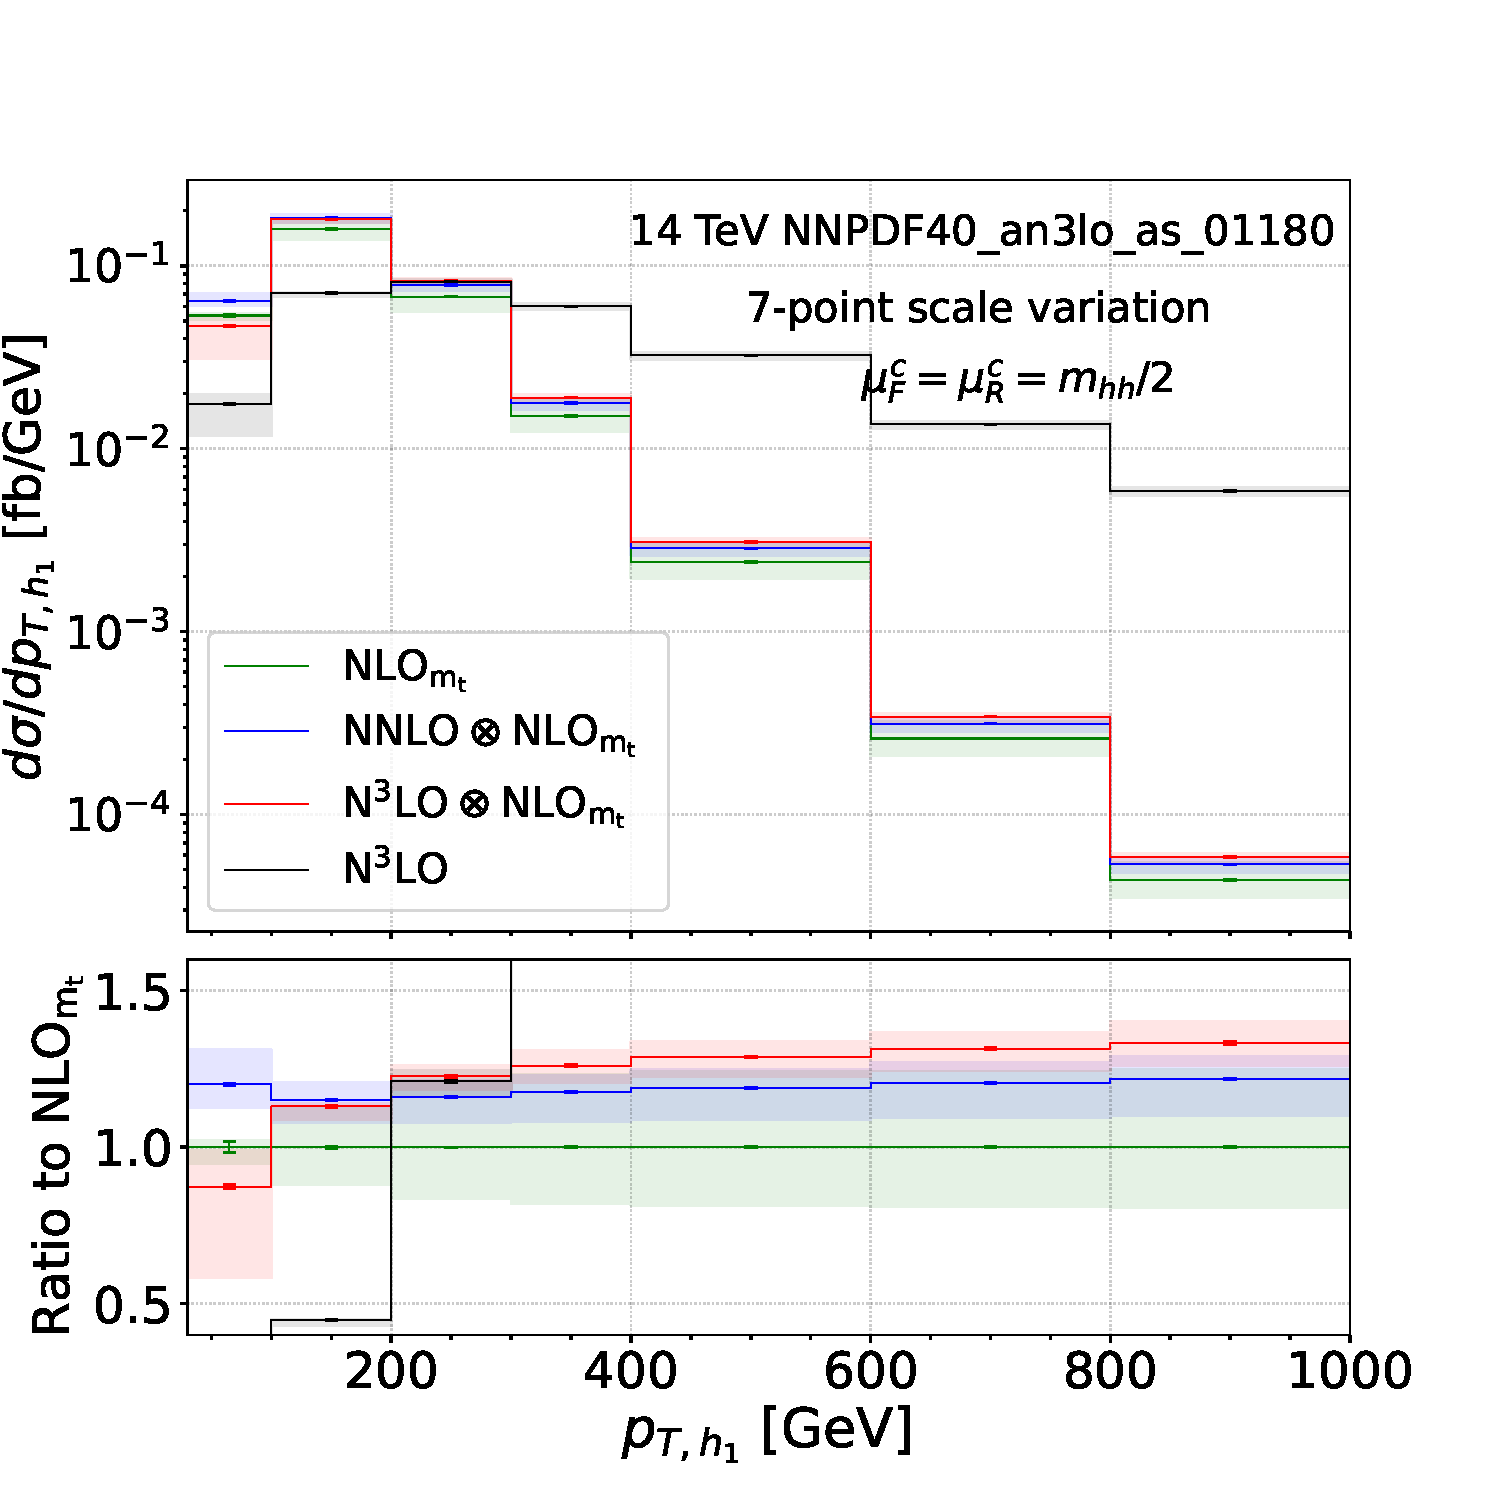
\includegraphics[width=0.49\textwidth,height=7.52cm]{N3LO_QCD_SM/N3LO_mt/Images/HH_pt_h1st_r.pdf}
\caption{Inclusive (left) and fiducial (right) leading-Higgs $p_{T}$ distributions for Higgs boson pair production at $\sqrt{s}=14$ TeV, including top quark mass effects. The error bands stem from $7$-point scale variations. Here $\mu^C$ denotes the central value of the renormalization and factorization scales. Results shown are from Ref.~\cite{Chen:2026zmi}.}
\label{fig:fid_pth1_mt}
\end{figure*}


\begin{figure*}[h]
\centering
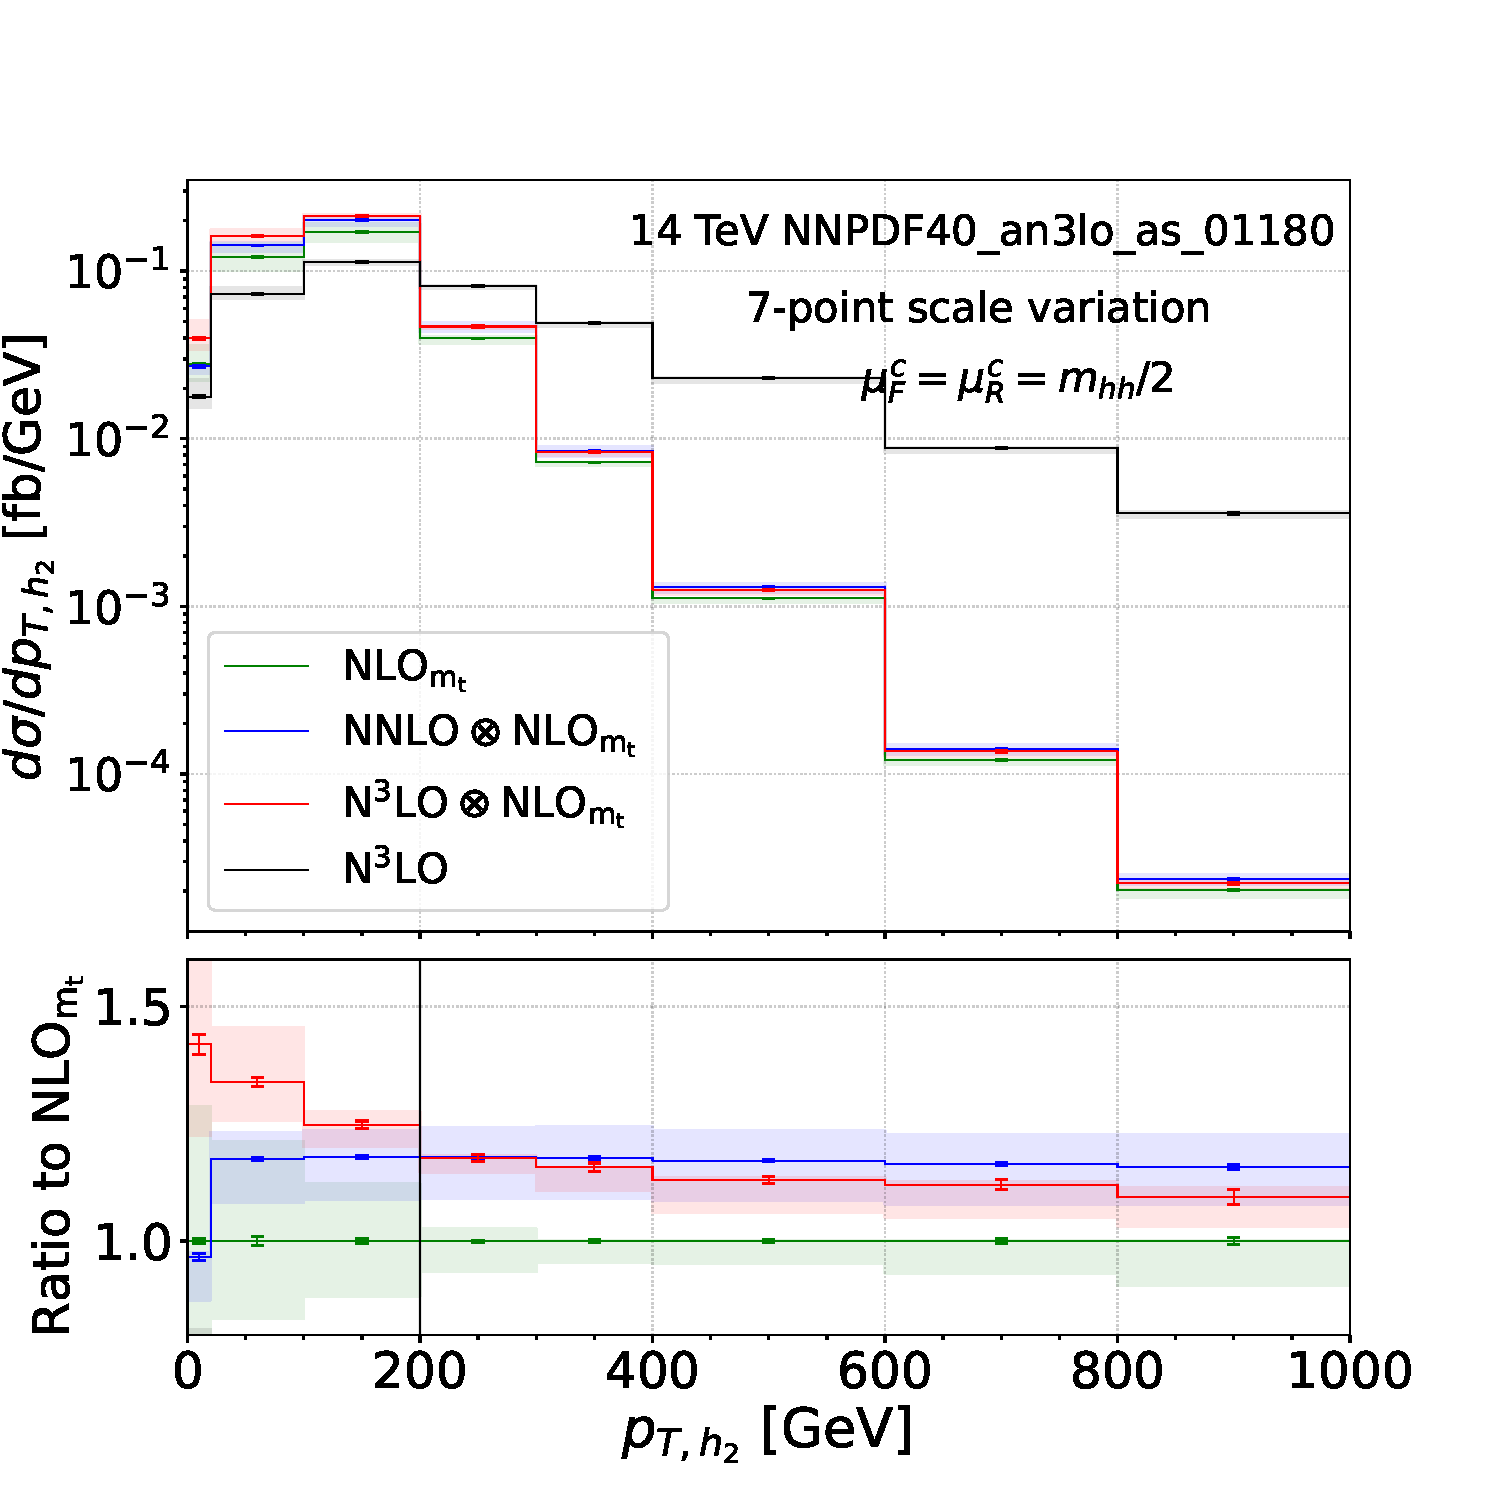
\includegraphics[width=0.49\textwidth,height=7.52cm]{N3LO_QCD_SM/N3LO_mt/Images/HH_pt_h2nd_100_r.pdf}
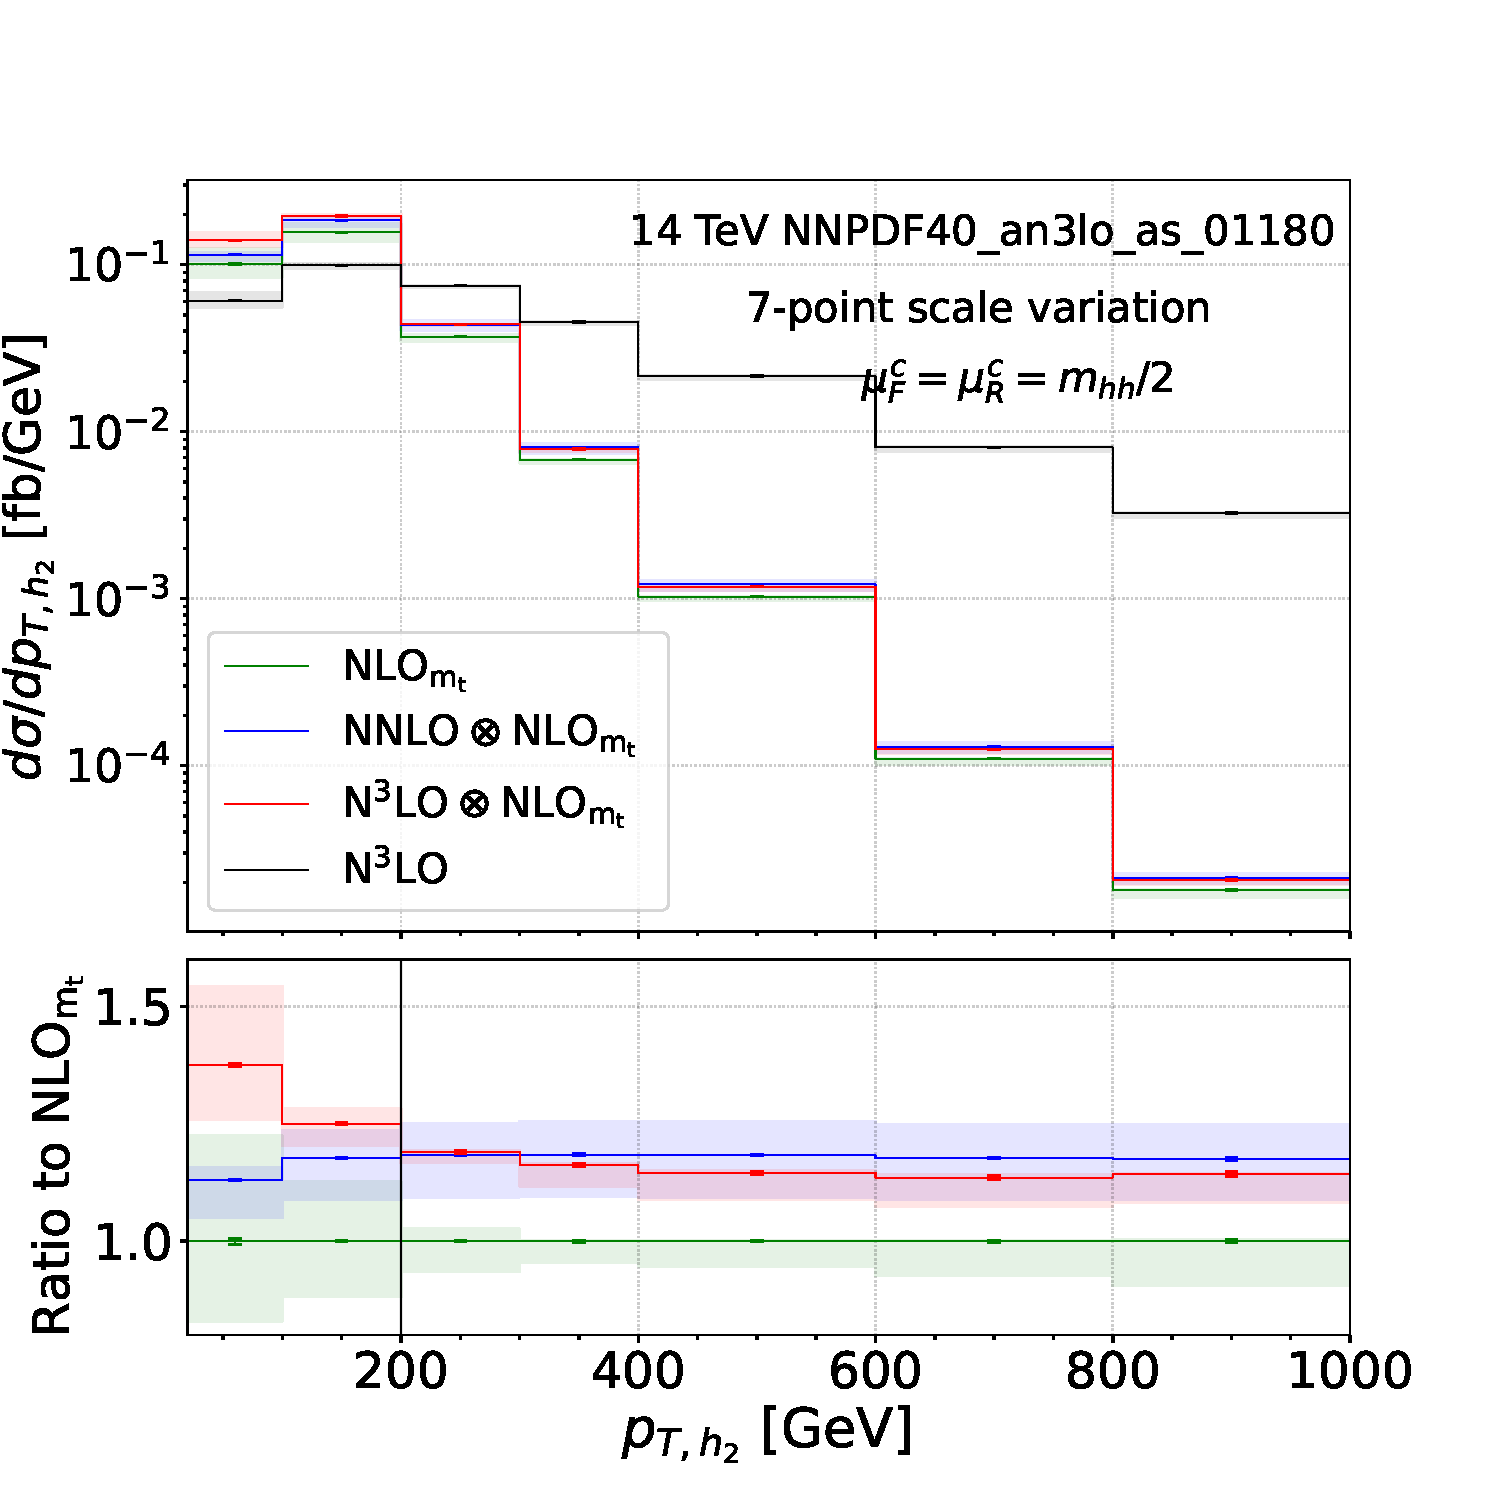
\includegraphics[width=0.49\textwidth,height=7.52cm]{N3LO_QCD_SM/N3LO_mt/Images/HH_pt_h2nd_r.pdf}
\caption{Inclusive (left) and fiducial (right) subleading-Higgs $p_{T}$ distributions for Higgs boson pair production at $\sqrt{s}=14$ TeV, including top quark mass effects. The error bands stem from $7$-point scale variations. Here $\mu^C$ denotes the central value of the renormalization and factorization scales. Results shown are from Ref.~\cite{Chen:2026zmi}.}
\label{fig:fid_pth2_mt}
\end{figure*}
